\section*{Chapter 11}

\subsection*{Exercise 11.1}

Convert the equation of $n$-step off-policy TD (7.9) to semi-gradient form.
Give accompanying definitions of the return for both the episodic and continuing cases.

\subsection*{Solution}

(7.9) is the following equation:

\[
    V_{t+n}(S_t) = V_{t+n-1}(S_t) + \alpha \rho_{t:t+n-1} [G_{t:t+n} - V_{t+n-1}(S_t)].
\]

The semi-gradient form of this equation is:

\[
    \mathbf{w}_{t+n} = \mathbf{w}_{t+n-1} + \alpha \rho_{t:t+n-1} \left[G_{t:t+n} - \hat{v}(S_t,\mathbf{w}_{t+n-1}) \right] \nabla \hat{v}(S_t,\mathbf{w}_{t+n-1}).
\]

With the following definitions of the return:

\begin{align*}
    G_{t:t+n} &\doteq R_{t+1} + \gamma R_{t+2} + \ldots + \gamma^{n-1} R_{t+n} + \gamma^n \hat{v}(S_{t+n},\mathbf{w}_{t+n-1}), \text{\qquad (episodic)}\\
    G_{t:t+n} &\doteq R_{t+1} - \bar{R}_{t} + \ldots +  R_{t+n} - \bar{R}_{t+n-1}  +  \hat{v}(S_{t+n},\mathbf{w}_{t+n-1}) \text{\qquad (continuing).}
\end{align*}


\subsection*{*Exercise 11.2}

Convert the equations of $n$-step $Q(\sigma)$ (7.11 and 7.17) to semi-gradient
form. Give definitions that cover both the episodic and continuing cases. 

\subsection*{Solution}
(7.11) is the following equation:

\[
    Q_{t+n}(S_t, A_t) = Q_{t+n-1}(S_t, A_t) + \alpha \rho_{t+1:t+n} [G_{t:t+n} - Q_{t+n-1}(S_t, A_t)].
\]

The semi-gradient form of this equation is:

\[
    \mathbf{w}_{t+n} \doteq \mathbf{w}_{t+n-1} + \alpha \rho_{t+1:t+n}\left[G_{t:t+n} - \hat{q}(S_t, A_t, \mathbf{w}_{t+n-1})\right]\nabla \hat{q}(S_t,A_t,\mathbf{w}_{t+n-1}).
\]

With the following definitions of the return:
{\scriptsize 
\begin{align*}
    G_{t:t+n} \doteq R_{t+1} &+ \gamma \left( \sigma_{t+1} \rho_{t+1} + (1 - \sigma_{t+1}) \pi(A_{t+1} \mid S_{t+1}) \right) \left( G_{t+1:t+n} - \hat{q}(S_{t+1}, A_{t+1},\mathbf{w}_{t+n-1}) \right) \\
    &+ \gamma \sum_a \pi(a \mid S_{t+1}) \hat{q}(S_{t+1}, a,\mathbf{w}_{t+n-1}) \text{\quad (episodic)}\\
    G_{t:t+n} \doteq R_{t+1} &- \bar{R}_{t} + \gamma \left( \sigma_{t+1} \rho_{t+1} + (1 - \sigma_{t+1}) \pi(A_{t+1} \mid S_{t+1}) \right) \left( G_{t+1:t+n} - \hat{q}(S_{t+1}, A_{t+1},\mathbf{w}_{t+n-1}) \right) \\
    &+ \gamma \sum_a \pi(a \mid S_{t+1}) \hat{q}(S_{t+1}, a,\mathbf{w}_{t+n-1}) \text{\quad (continuing)}
\end{align*}
}
\subsection*{Exercise 11.3 (programming)}

Apply one-step semi-gradient Q-learning to Baird's counterexample and show empirically that its weights diverge. 

\subsection*{Solution}
See the notebook.
\begin{figure}[H]
    \centering
    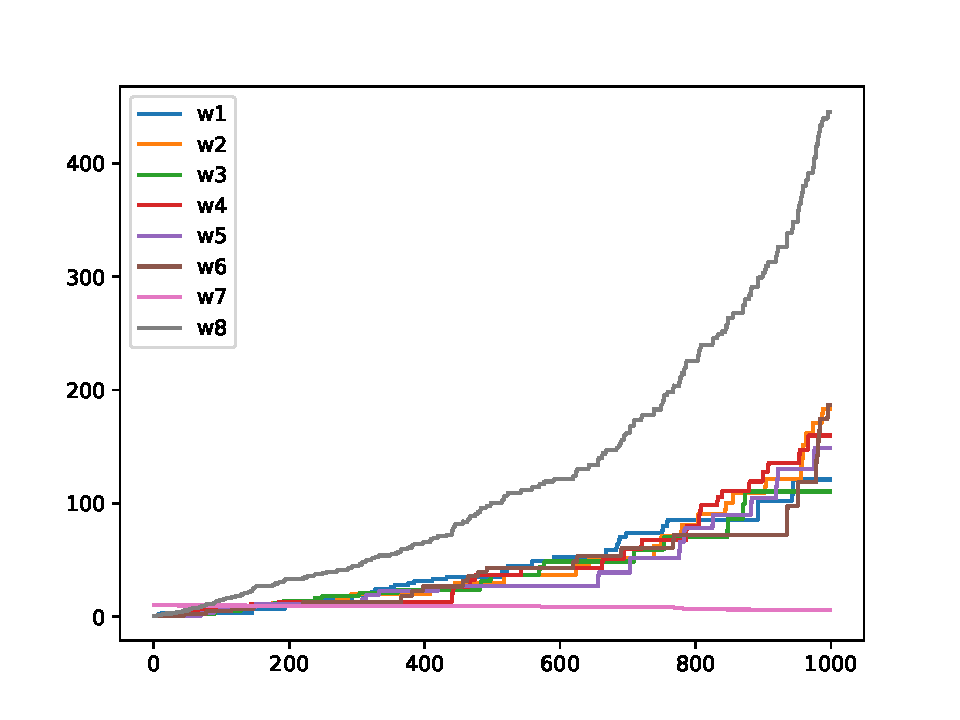
\includegraphics[width=0.9\textwidth]{chapters_latex/figures/ex_11_03.pdf}
    \captionsetup{labelformat=empty}
\end{figure}

\subsection*{*Exercise 11.4}

Prove (11.24). Hint: Write the $\overline{\text{RE}}$ as an expectation over possible states
$s$ of the expectation of the squared error given that $S_t = s$. Then add and subtract the
true value of state $s$ from the error (before squaring), grouping the subtracted true value
with the return and the added true value with the estimated value. Then, if you expand
the square, the most complex term will end up being zero, leaving you with (11.24).

\subsection*{Solution}

\begin{align*}
    \overline{\text{RE}} &= \mathbb{E} \left[ \left( G_t - \hat{v}(S_t,\mathbf{w}) \right)^2 \right] \\
    &= \mathbb{E}_s \left[ \mathbb{E} \left[ \left(G_t -  \hat{v}(S_t,\mathbf{w}) \right)^2 \mid S_t = s \right] \right] \\
    &= \mathbb{E}_s \left[ \mathbb{E} \left[ \left(G_t - V^\pi(S_t) + V^\pi(S_t) - \hat{v}(S_t,\mathbf{w}) \right)^2 \mid S_t = s \right] \right] \\
    &= \mathbb{E}_s \Big[ \mathbb{E} \Big[ \left(G_t - V^\pi(S_t) \right)^2 
    + 2 \left(G_t - V^\pi(S_t) \right) \left(V^\pi(S_t) - \hat{v}(S_t,\mathbf{w}) \right)  \\
    &\quad + \left(V^\pi(S_t) - \hat{v}(S_t,\mathbf{w}) \right)^2 \mid S_t = s \Big] \Big] \\
    &= \mathbb{E}_s \Big[\mathbb{E} \left[ \left(G_t - V^\pi(s)\right)^2 \mid S_t = s \right] \\
    &\quad + 2 \mathbb{E} \left[ G_t - V^\pi(s) \mid S_t = s \right] (V^\pi(s) - \hat{v}(S_t,\mathbf{w})) \\
    &\quad + \mathbb{E}\left[ (V^\pi(s) - \hat{v}(S_t,\mathbf{w}))^2 \mid S_t = s \right] \Big] \\
    &= \mathbb{E}_s \left[\mathbb{E} \left[ \left(G_t - V^\pi(s)\right)^2 \mid S_t = s \right] + \mathbb{E}\left[ \left(V^\pi(s) - \hat{v}(S_t,\mathbf{w})\right)^2 \mid S_t = s \right] \right] \\
    &= \mathbb{E} \left[ \left(G_t - V^\pi(s)\right)^2 \right] +  \overline{VE}.
\end{align*}

